\documentclass[12pt, a4paper]{article}

\usepackage[a4paper, ]{geometry}
\usepackage{graphicx} % Required for inserting images
\usepackage{array}
\usepackage{multirow}
\usepackage{float}

\usepackage[czech]{babel}
\usepackage{hyperref}
\usepackage{amsmath}
\usepackage{sectsty}
\usepackage{gensymb}

\usepackage{subfigure}

\usepackage{matlab-prettifier}

\RequirePackage[inner=1cm,outer=1cm,top=2cm,bottom=1cm]{geometry}

\renewcommand{\baselinestretch}{1.25}
\newcommand\tab[1][0.7cm]{\hspace*{#1}}

\title{Technická zpráva}
\date{}

\begin{document}

    \pagestyle{empty}
    % Autor [2023]: Tereza Černohousová
% Upravil [2023]: Matyáš Pokorný
% Upravil [2024]: Filip Roučka
% Upravil [2025]: Michal Kovář

% Doporučené balíčky:
% \usepackage[czech]{babel} % Pro podporu českého jazyka
% \usepackage[utf8]{inputenc} % Nastavení kódování na UTF8
% \usepackage[T1]{fontenc} % Zajištění správného kopírování textu s českou diakritikou
% \usepackage{tikz} % Pro kreslení grafiky
% \usepackage{hhline} % Pro pokročilé čáry v tabulkách
% \usepackage{datetime} % Pro práci s datem

\newgeometry{left=2cm, right=2cm, top=2cm, bottom=2cm}

\newdateformat{czechdate}{\THEDAY. \THEMONTH. \THEYEAR} % Formátování data
\renewcommand{\baselinestretch}{1.5} % Nastavení řádkování na 1.5
\vspace*{\fill} % Posunutí tabulky více ke spodní části stránky

\begin{center}
\centering
\tikz\node[draw=black,inner sep=2pt, anchor=center] {
\begin{tabular}{|clllllll|}
\hline
\multicolumn{8}{|c|}{\vspace{-0.5cm}\small}\\
\multicolumn{8}{|c|}{\Large\textbf{ČESKÉ VYSOKÉ UČENÍ TECHNICKÉ V PRAZE}}\\
\multicolumn{8}{|c|}{\large FAKULTA STAVEBNÍ, OBOR GEODÉZIE A KARTOGRAFIE}\\
\multicolumn{8}{|c|}{\large KATEDRA GEOMATIKY}\\
\hhline{========}
\multicolumn{8}{|l|}{\raggedright\small\textbf{Název předmětu:}} \\
\multicolumn{8}{|c|}{\raggedright\textbf{VTTG - Výuka v terénu z teoretické geodézie}} \\
\hline
\multicolumn{1}{|l|}{\raggedright\small\textbf{Úloha:}} & \multicolumn{7}{|l|}{\raggedright\small\textbf{Název úlohy:}} \\
\multicolumn{1}{|c|}{\raggedright\text{TRG}} & \multicolumn{7}{|c|}{\raggedright Triangulace a trilaterace na velké vzdálenosti} \\
\hline
\multicolumn{1}{|l|}{\raggedright\small\textbf{Akademický rok:}} & \multicolumn{1}{c|}{\raggedright\small\textbf{Semestr:}} & \multicolumn{1}{l|}{\raggedright\small\textbf{Skupina:}} & \multicolumn{1}{c|}{\raggedright\small\textbf{Vypracoval:}} & \multicolumn{1}{l|}{\raggedright\small\textbf{Datum:}} & \multicolumn{3}{l|}{\raggedright\small\textbf{Klasifikace:}} \\
\multicolumn{1}{|l|}{} & \multicolumn{1}{c|}{} & \multicolumn{1}{l|}{} & \multicolumn{1}{c|}{Josef Bořík, Matěj Klimeš} & \multicolumn{1}{l|}{} & \multicolumn{3}{l|}{} \\
\multicolumn{1}{|l|}{} & \multicolumn{1}{c|}{} & \multicolumn{1}{l|}{} & \multicolumn{1}{c|}{Michal Kovář, Matyáš Pokorný} & \multicolumn{1}{l|}{} & \multicolumn{3}{l|}{} \\
\multicolumn{1}{|c|}{2024/2025} & \multicolumn{1}{c|}{letní} & \multicolumn{1}{c|}{1} & \multicolumn{1}{c|}{Filip Roučka, Kryšof Sedlák} & \multicolumn{1}{l|}{\czechdate\today} & \multicolumn{3}{l|}{} \\
\hline
\end{tabular}
};
\end{center}
\thispagestyle{empty}

\renewcommand{\baselinestretch}{1} % Nastavení řádkování zpět na 1
\newgeometry{left=25.4mm, right=25.4mm, top=25.4mm, bottom=25.4mm}
    \pagestyle{plain}
    \setcounter{page}{1}
    
    \maketitle
    
    \section{Zadání}
    \section{Zadání}

Cílem této úlohy je obnova a nové zaměření části nivelačního pořadu II. řádu Z7ab Žleb–Kunčice, konkrétně v úseku Nová Seninka – Kladské sedlo, metodou velmi přesné nivelace (VPN). V rámci obnovy mají být provedeny následující činnosti:
\begin{itemize}
    \item v případě potřeby zřízení nových nivelačních bodů;
    \item určení převýšení jednotlivých oddílů metodou velmi přesné nivelace (VPN) za použití digitálního nivelačního přístroje Leica a nivelačních latí s čárovým kódem;
    \item převedení měřených převýšení do výškového systému Bpv (Baltský po vyrovnání);
    \item vytvoření kompletních nivelačních údajů pro všechny body daného měřeného úseku.
\end{itemize}
Součástí zpracování úlohy je rovněž gravimetrické měření na vybraných bodech, které umožní výpočet normálních výšek a tíhových anomálií.

    \newpage

    \section{Informace o měření}
    \section{Informace o měření}
\setstretch{1.5} % řádkování
\begin{tabular}{lll} 
\textit{Místo měření:} & & Staré Město pod Sněžníkem a okolí (okres Šumperk)\\ 
\textit{Datum měření:} & & 13.~6.~2025 – triangulace, trilaterace, astro měření;\\
& & 14.~6.~2025 – měření gyroteodolitem, sk č. 3\\
& & 16.~6.~2025 – měření gyroteodolitem, sk č. 1\\
\textit{Povětrnostní podmínky:} & & 13.~6.~2025 – jasno, slabý vítr, teplota cca 20–24°C\\
 & & 14.~6.~2025 – jasno, mírný vítr, teplota cca 20–24~°C \\
 & & 16.~6.~2025 – zataženo, deštivo,  teplota cca 17–20~°C.\\
\textit{Použité přístroje a pomůcky:} & & 2× totální stanice Leica TC1700 / Topcon GPT‑7501,\\
& & souprava hranolů (centrické a excentrické), minihranol,\\
& & 2× stativ, 2× měřická lať,\\
& & gyroteodolit, stopky, přijímač pro čas UTC,\\
& & meteorologická souprava (teploměr, vlhkoměr, barometr)\\
\textit{Souřadnicový systém:} & & S‑JTSK\\ 
\end{tabular}


    \newpage

    %\section{Pomůcky}
    %\begin{itemize}
    \item 3 x Leica Sprinter 100, v.č.: 738932, 1007227, 1007439
    \item 2 x Trimble TRMR2, v.č.: 32S17769, 6203S17886
    \item Trimble TRMR580, 6337S22116
    \item nivelační latě
    \item kladivo
    \item svinovací metr
    \item nivelační podložky
    \item dřevěné kolíky
    \item stativy
\end{itemize}



    %\newpage

    \section{Pracovní postup - Zpracování měření}
    
\subsection{Měření GNSS}

\tab Měření GNSS probíhalo rychlou statickou metodou s použitím referenční stanice ve Starém Městě (TSTA). Data z měření byla exportována do formátu RINEX. Byla použita observační data ze stanice CZEPOS v Šumperku (CSUM).

Zpracování bylo provedeno v programu RTKLib. 

\subsection{Technická nivelace}

\tab Nivelace byla použita pro určení výšky bodu z excentrického stanoviska, s maximem dvou přestav.

Hodnocení přesnosti nivelace porovnáním rozdílů nivelovaných převýšení a mezní odchylkou probíhalo už v terénu podle:

\begin{equation}
    \Delta M_{[mm]}=0,67*40*\sqrt{R_{[km]}},
\end{equation}

kde $R_{[km]}$ je délka pořadu v kilometrech.\\

Vyhovující dvojice měření pak byla zprůměrována.\\

Přesnost měření popisuje střední jednotková chyba kilometrová obousměrné nivelace:

\begin{equation}
    m_{0[mm]}=\frac{1}{2}\sqrt{\frac{\delta h}{R_{[km]}}},
\end{equation}

směrodatná odchylka nivelovaného převýšení:

\begin{equation}
    m_{[mm]}=m_0\sqrt{R_{[km]}},
\end{equation}

a její mezní hodnota:

\begin{equation}
    m_{[mm]}=1,00 + \frac{1,77}{\sqrt{M}},
\end{equation}

kde $M$ je počet oddílů v pořadu.

Výšky měřené dvěma skupinami byly zprůměrovány a ze zákona hromadění směrodatných odchylek je směrodatná odchylka průměru:

\begin{equation}
    \sigma_{\varnothing m}=2\sqrt{\sigma_{m1}^2+\sigma_{m2}^2}.
\end{equation}

\subsection{Výpočet výškové anomálie}

\tab Výšková anomálie je rozdíl elipsoidické (určené GNSS) a normální Moloděnského výšky (určené nivelací): 

\begin{equation}
    N=H_{el}-H_{niv}.
\end{equation}

Její přesnost je ze zákona hromadění směrodatných odchylek:

\begin{equation}
    \sigma_N=\sqrt{\sigma_{Hel}^2+\sigma_{Hniv}^2}.
\end{equation}


    \newpage
    
    \section{Výsledky}
    % --- ŽLUTÁ – Souřadnice a výšky ---
\begin{table}[H]
\centering
\caption{Souřadnice a výšky, Staré Město - Nová Seninka}
%\resizebox{\textwidth}{!}{
\begin{tabular}{l|rrrr}
\hline
Bod & B[°] & L[°] & H[m] & $\sigma_H$ [mm] \\
\hline
  23K & 50,16409 & 16,94625 & 568,281 & 19,0 \\
  25K & 50,16751 & 16,94516 & 582,711 & 19,0 \\
27.1K & 50,17650 & 16,93953 & 588,495 & 19,0 \\
  29K & 50,17916 & 16,93285 & 598,338 & 19,0 \\
  30K & 50,18047 & 16,92536 & 610,191 & 19,0 \\
  31K & 50,18666 & 16,92124 & 624,857 & 19,0 \\
31.1K & 50,19064 & 16,91935 & 635,698 & 19,0 \\
  32K & 50,19339 & 16,91916 & 643,479 & 19,0 \\
\hline
\end{tabular}
\end{table}

\begin{table}[H]
\centering
\caption{Souřadnice a výšky, Nová Seninka - Kladské Sedlo}
\resizebox{\textwidth}{!}{
\begin{tabular}{l|rrrr|rrrr}
\hline
\multicolumn{4}{c}{\textbf{Sk.1}} & \multicolumn{4}{c}{\textbf{Sk.2}} \\
Bod & B[°] & L[°] & H[m] &$\sigma_H$[mm]& B[°] & L[°] & H[m] &$\sigma_H$[mm]\\
\hline
33.1K & 50,19856 & 16,91752 & 658,562 &  9.3 & 50,19856 & 16,91752 & 658,581 & 5.1 \\
34K   & 50,20344 & 16,91535 & 676,095 &  2.9 & 50,20344 & 16,91535 & 676,089 & 1.0 \\
35.1B & 50,20855 & 16,91942 & 699,480 & 24.0 & 50,20855 & 16,91942 & 699,432 &   0 \\
36.1B & 50,21102 & 16,92066 & 711,668 & 18.0 & 50,21102 & 16,92066 & 711,704 &   0 \\
37K   & 50,21610 & 16,92155 & 740,612 & 43.0 & 50,21610 & 16,92155 & 740,698 & 0.0 \\
39.1K & 50,21817 & 16,92567 & 771,620 & 18.1 & 50,21817 & 16,92567 & 771,657 & 0.0 \\
43K   & 50,21969 & 16,92524 & 828,388 & 29.4 & 50,21969 & 16,92524 & 828,447 & 1.0 \\
44K   & 50,22303 & 16,92363 & 845,421 &  7.6 & 50,22303 & 16,92363 & 845,406 & 1.4 \\
\hline
\end{tabular}}
\end{table}


% --- ŽLUTÁ – Výsledky měření ---
\begin{table}[H]
\centering
\caption{Výsledky měření, Staré Město - Nová Seninka}
%\resizebox{\textwidth}{!}{
\begin{tabular}{l|rrrrr}
\hline
Bod & $H_{niv}$[m] & $m_0$[mm] & $m$[mm] & $H_{el}$[m] & $\sigma_{Hel}$ [mm]\\
\hline
  23K & 524,507 & 0,0 & 0,0 & 568,281 & 19,0\\
  25K & 538,941 & 0,0 & 0,0 & 582,711 & 19,0\\
27.1K & 544,738 & 5,0 & 1,0 & 588,495 & 19,0\\
  29K & 554,575 & 4,2 & 0,5 & 598,338 & 19,0\\
  30K & 566,417 & 0,0 & 0,0 & 610,191 & 19,0\\
  31K & 581,028 & 3,0 & 0,5 & 624,857 & 19,0\\
31.1K & 591,914 & 2,2 & 0,5 & 635,698 & 19,0\\
  32K & 599,737 & 0,0 & 0,0 & 643,479 & 19,0\\
\hline
\end{tabular}
\end{table}

% --- ZELENÁ + MODRÁ – Výsledky měření ---
\begin{table}[H]
\centering
\caption{Výsledky měření, Nová Seninka - Kladské Sedlo}
\resizebox{\textwidth}{!}{
\begin{tabular}{l|rrrr|rrrr|r}
\hline
\multicolumn{4}{c}{\textbf{Sk.1}} & \multicolumn{4}{c}{\textbf{Sk.2}}  & \\
Bod & $H_{niv}[m]$ & $m[mm]$ & $H_{el}[m]$ & $\sigma_{Hel}[mm]$ & $H_{niv}[m]$ & $m[mm]$ & $H_{el}[m]$ & $\sigma_{Hel}[mm]$ & $\Delta H_{el}[m]$ \\
\hline
33.1K & 614,854 & 0,5 & 658,562 &  9.3 & 614,853 & 2,5 & 658,581 & 5.1 &  0,019 \\
34K   & 632,371 & 0,0 & 676,095 &  2.9 & 632,371 & 0,5 & 676,089 & 1.0 & -0,006 \\
35.1B & 655,705 & $-$ & 699,480 & 24.0 & 655,705 & $-$ & 699,432 &   0 & -0,048 \\
36.1B & 667,927 & $-$ & 711,668 & 18.0 & 667,927 & $-$ & 711,704 &   0 &  0,036 \\
37K   & 696,922 & 0,0 & 740,612 & 43.0 & 696,922 & 0,0 & 740,698 & 0.0 &  0,086 \\
39.1K & 727,931 & 0,0 & 771,620 & 18.1 & 727,930 & 0,0 & 771,657 & 0.0 &  0,037 \\
43K   & 784,740 & 0,0 & 828,388 & 29.4 & 784,740 & 0,5 & 828,447 & 1.0 &  0,059 \\
44K   & 801,798 & 0,5 & 845,421 &  7.6 & 801,797 & 0,5 & 845,406 & 1.4 & -0,015 \\
\hline
\end{tabular}}
\end{table}


% --- PRŮMĚR – Souřadnice a výšky ---
\begin{table}[H]
\centering
\caption{PRŮMĚR – Souřadnice a výšky, Staré Město - Kladské Sedlo}
%\resizebox{\textwidth}{!}{
\begin{tabular}{l|rrrr}
\hline
Bod & B[°] & L[°] & H[m] & $\sigma_H$[mm] \\
\hline
  23K & 50,16409 & 16,94625 & 568,281 & 19,0 \\
  25K & 50,16751 & 16,94516 & 582,711 & 19,0 \\
27.1K & 50,17650 & 16,93953 & 588,495 & 19,0 \\
  29K & 50,17916 & 16,93285 & 598,338 & 19,0 \\
  30K & 50,18047 & 16,92536 & 610,191 & 19,0 \\
  31K & 50,18666 & 16,92124 & 624,857 & 19,0 \\
31.1K & 50,19064 & 16,91935 & 635,698 & 19,0 \\
  32K & 50,19339 & 16,91916 & 643,479 & 19,0 \\
33.1K & 50,19856 & 16,91752 & 658,571 &  9,3 \\
  34K & 50,20344 & 16,91535 & 676,092 &  2,9 \\
35.1B & 50,20855 & 16,91942 & 699,456 & 24,0 \\
36.1B & 50,21102 & 16,92066 & 711,686 & 18,0 \\
  37K & 50,21610 & 16,92155 & 740,655 & 43,0 \\
39.1K & 50,21817 & 16,92567 & 771,638 & 18,1 \\
  43K & 50,21969 & 16,92524 & 828,418 & 29,4 \\
  44K & 50,22303 & 16,92363 & 845,414 &  7,6 \\
\hline
\end{tabular}
\end{table}

% --- PRŮMĚR – Výsledky měření ---
\begin{table}[H]
\centering
\caption{PRŮMĚR – Výsledky měření, Staré Město - Kladské Sedlo}
\resizebox{\textwidth}{!}{
\begin{tabular}{l|rrrrrrrrr}
Bod & $H_{niv}[m]$ & $m[mm]$ & $H_{el}[m]$ & $\sigma_{Hel}[mm]$ & $N_{int}[m]$ & $N[m]$ & $N_{int}-N[m]$ & $\sigma_N[mm]$ \\
\hline
  23K & 524,507 & 0,0 & 568,281 & 19,0 & 43.805 & 43.774 &  0.031 &   0.0 &\\
  25K & 538,941 & 0,0 & 582,711 & 19,0 & 43.795 & 43.770 &  0.025 &   0.0 &\\
27.1K & 544,738 & 1,0 & 588,495 & 19,0 & 43.790 & 43.757 &  0.033 &   2.0 &\\
  29K & 554,575 & 0,5 & 598,338 & 19,0 & 43.790 & 43.763 &  0.027 &   1.0 &\\
  30K & 566,417 & 0,0 & 610,191 & 19,0 & 43.790 & 43.774 &  0.015 &   0.0 &\\
  31K & 581,028 & 0,5 & 624,857 & 19,0 & 43.784 & 43.829 & -0.045 &   1.0 &\\
31.1K & 591,914 & 0,5 & 635,698 & 19,0 & 43.779 & 43.784 & -0.004 &   1.0 &\\
  32K & 599,737 & 0,0 & 643,479 & 19,0 & 43.776 & 43.742 &  0.033 &   0.0 &\\
33.1K & 614,854 & 5,1 & 658,571 &  9,3 & 43.769 & 43.718 &  0.051 &  10.6 &\\
  34K & 632,371 & 1,0 & 676,092 &  2,9 & 43.738 & 43.721 &  0.017 &   3.0 &\\
35.1B & 655,705 & $-$ & 699,456 & 24,0 & 43.728 & 43.751 & -0.022 &  24.0&\\
36.1B & 667,927 & $-$ & 711,686 & 18,0 & 43.722 & 43.759 & -0.036 &  18.0&\\
  37K & 696,922 & 0,0 & 740,655 & 43,0 & 43.707 & 43.733 & -0.025 &  43.0  &\\
39.1K & 727,931 & 0,0 & 771,638 & 18,1 & 43.682 & 43.708 & -0.025 &  18.1  &\\
  43K & 784,740 & 1,0 & 828,418 & 29,4 & 43.673 & 43.678 & -0.004 &  29.4 &\\
  44K & 801,798 & 1,4 & 845,414 &  7,6 & 43.658 & 43.616 &  0.042 &   7.0 &\\
\hline
\end{tabular}}
\label{prum}
\end{table}

%c_bodu_vec N_vec N_mervec N_vec-N_mervec sigma_vec

%    23     43.805    43.774     0.031528          0
%    25     43.795    43.770     0.02529           0
%  27.1      43.79    43.757     0.03337           2
%    29      43.79    43.763     0.027033          1
%    30      43.79    43.774     0.015611          0
%    31     43.784    43.829    -0.045588          1
%  31.1     43.779    43.784    -0.0042041         1
%    32     43.776    43.742     0.033835          0
%  33.1     43.769    43.718     0.051636         10.607
%    34     43.738    43.721     0.017257          3.0676
%  35.1     43.728    43.751    -0.022964         24
%  36.1     43.722    43.759    -0.03698          18
%    37     43.707    43.733    -0.025462         43
%  39.1     43.682    43.708    -0.025622         18.1
%    43     43.673    43.678    -0.0046542       29.417
%    44     43.658    43.616     0.042092         7.7279

\begin{figure}[H]
    \centering
    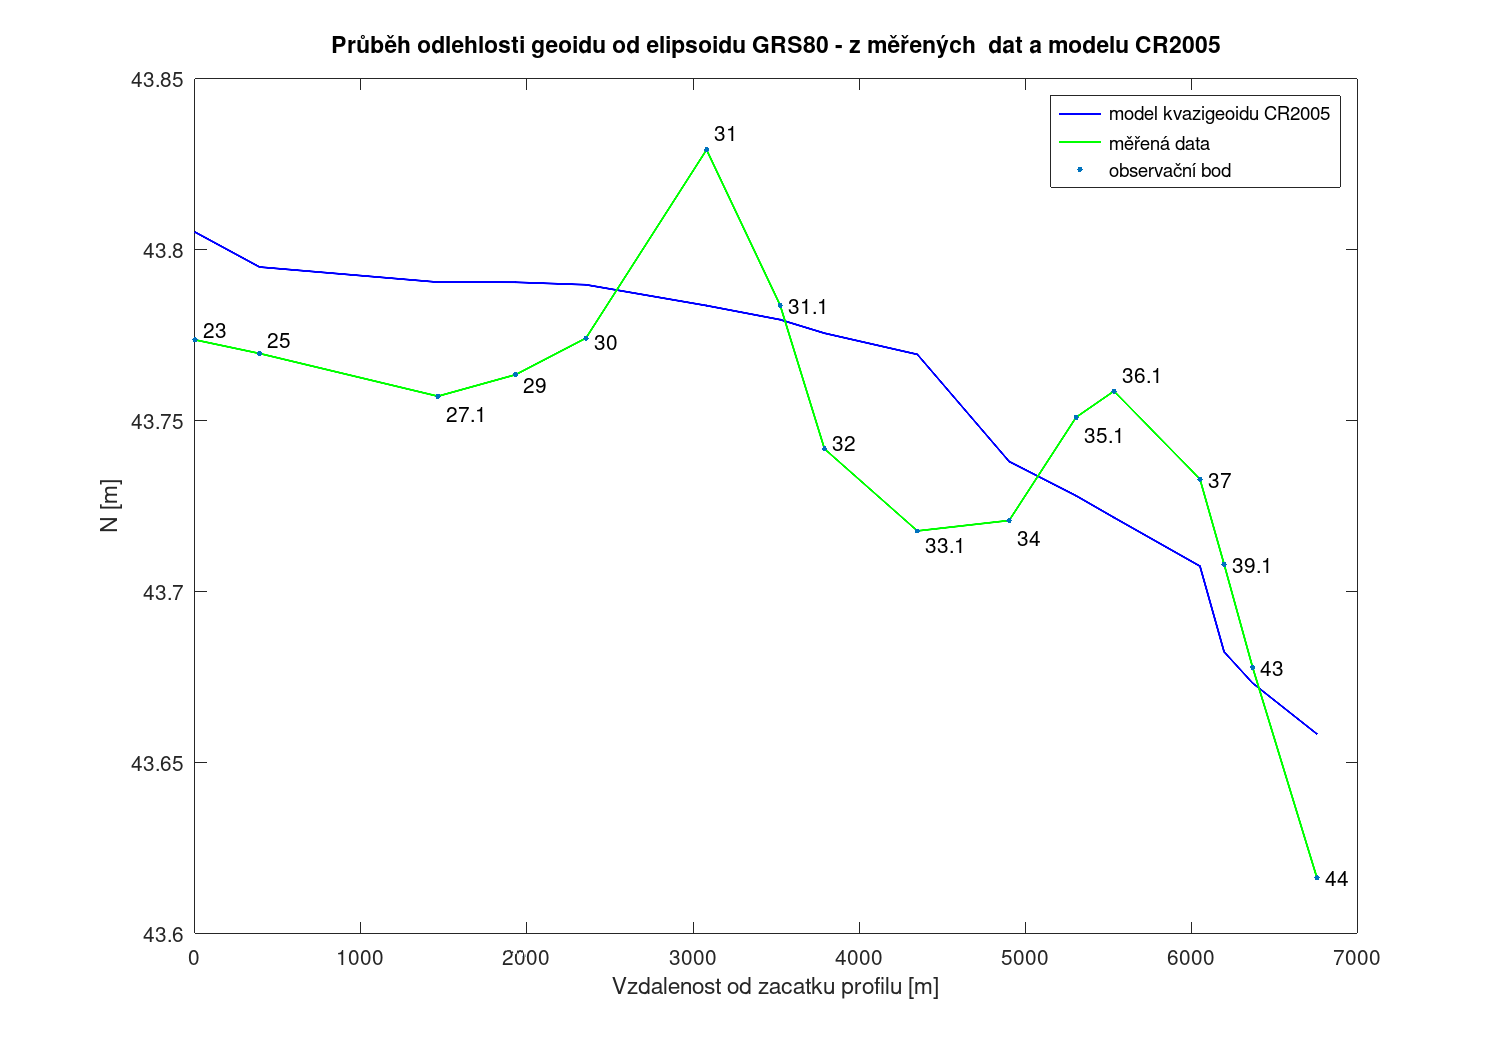
\includegraphics[width=15cm]{graf_profil.png}
    \caption{Grafické znázornění průběhu kvazigeoidu na zadaném profilu}
    \label{fig:enter-label}
\end{figure}


    \newpage

    \section{Závěr}
    \tab  V rámci této úlohy byl stanoven průběh kvazigeoidu v profilu podél nivelačního pořadu II. řádu Z7ab, konkrétně v úseku od Vysoké Žibřidovice po Kladské sedlo. Bylo provedeno GNSS měření pro určení elipsoidických výšek v systému ETRS89 a technická nivelace pro stanovení normálních výšek v systému Bpv. Byla vypočtena výšková anomálie kvazigeoidu pro jednotlivé body profilu.

Naměřené hodnoty byly následně porovnány s hodnotami modelu kvazigeoidu CR2005. Získané výsledky prokázaly, že model CR2005 se v dané oblasti blíží skutečnému průběhu kvazigeoidu. Rozdíly mezi naměřenými a modelovými hodnotami jsou uvedeny v \ref{prum}, kde se pohybují v řádu milimetrů až centimetrů. Tyto odchylky jsou přijatelné vzhledem k použité metodice a přesnosti měření. 

Grafické znázornění průběhu výškových anomálií je na \ref{fig:enter-label}. 

    \section{Přílohy}
    \begin{enumerate}
    \item Protokol o vyrovnání sítě.
    \item Náčrt sítě (případně zákres do mapy).
    \item Protokol GNSS
\end{enumerate}



    
\vspace*{\fill}
\textbf{V Praze dne: .. 2025\hspace{5cm} M. Kovář, M. Pokorný,}

\textbf{\hspace{9.3cm}F. Roučka, K. Sedlák}

\newpage
\input{}


\end{document}



